Se incluye a continuación un resumen de la entrevista realizada el día 3 de diciembre de 2013 a los principales responsables del Área Informática del Ayuntamiento de Puerto Real y del Servicio de Recogida de Enseres y Limpieza. En ella nos encontramos presentes los siguientes participantes:
\begin{itemize}
\item Diego Rubio Abujas (entrevistador e ingeniero de requisitos).
\item Enrique Daneri (analista de sistema actual y responsable de la parte de aplicaciones).
\item Javier (actual responsable de la operativa de gestión de recogida de enseres).
\end{itemize}
 
La entrevista se inicia solicitando a los participantes su consentimiento para realizar la grabación de dicha entrevista. Se expone como motivo inicial de la entrevista, conocer el funcionamiento interno de la organización.
 
% EL PROCEDIMIENTO A SEGUIR
 
% Intervención del analista.
\paragraph{Enrique} Aunque dice no ser el responsable de la operativa, nos explica que se realizan una media de 20 recogidas diarias como máximo.  Nos comenta además que se realizan recogidas todos los días laborables. Es un solo camión el que realiza las recogidas actualmente. El proceso consiste en que el usuario realiza una llamada, el operador que recibe la llamada y tiene acceso a un registro de contenedores y actuales recogidas concertadas. El operador indica al usuario dónde debe depositar el elemento.  
\paragraph{} El proceso se realiza de la siguiente manera: hay una llamada del usuario y una vez recibida se le indica cuando debe depositar el mueble o el elemento a recoger. Si la fecha de recogida se prolonga más de 2 días, se ponen en contacto con el usuario para confirmar la recogida. 

\paragraph{}El analista nos da su punto de vista sobre la aplicación. La tecnología existente es efectuar una llamada a un operador y este proporciona la cita. Una forma de plantear la cita es indicar quien la solicita y que sea un operador el que la confirme. Hay un límite de muebles a recoger (3 muebles aproximadamente). Si se identifica el domicilio, la aplicación podía indicar las formas más próximas al domicilio del cliente. Se define dónde quiere el usuario que se recojan sus muebles, se queda a la espera de que se procese su solicitud, y finalmente se le da respuesta. 
 
\paragraph{}Otra opción que nos proporciona Enrique es: que la gestión se realice  de forma automatizada. Nos recuerda que se recogen enseres 20 diarios. Se comprueba que lo que solicita el usuario está dentro de los límites establecidos, se  indica la fecha en la que debe depositar los enseres al usuario. Se da opción de que el usuario solicite una fecha concreta. Una vez procesada la petición, el sistema da respuesta al usuario. Cuando llega el día de recogida, la aplicación podría enviar al usuario un recordatorio. Ocurre a veces que el mueble no se encuentre en el punto de recogida porque alguien haya pasado por el punto de recogida y se lo haya llevado. 
 
% Intervención del responsable de operativa.
\paragraph{Javier} Nos explica que hay una casuística muy grande tanto en tipos de muebles como en el incidencias ocurridas. Nos muestra su desacuerdo en automatizar el proceso de recogida. Nos expone diversos ejemplos: incrementos en el número de muebles por la suma de peticiones de recogidas no notificadas de los diversos vecinos del usuario, la problemática de no dejar los muebles en el lugar indicado, las negativas de los clientes a adaptarse al procedimiento de recogida (tanto en horario como en ubicación), etc. Finalmente nos expone que pocos usuarios realizan la gestión por vía telefónica (ya sea por desconocimiento del número o de la operativa a seguir), se expone la opción de ofrecer una idea alternativa para realizar la gestión mediante el lanzamiento de una aplicación móvil. Nos expone que el proceso no tiene ninguna problemática, la problemática está en la ejecución de la operativa y eso se escapa de la aplicación al ser por muchísimos factores humanos. El problema es de logística interna.
 
% Intervención del analista,
\paragraph{Enrique} Recalca que no es problema de la aplicación sino de logística interna. La dificultad está en la recogida, en cerrar el proceso.
 
% Intervención del responsable de operativa.
\paragraph{Javier} El usuario llama con el móvil y pide la cita, y la parte teórica no tiene problemas. Según él, el problema es cerrar el proceso, incluso con el método actual el operador tiene problemas en cerrar el trámite, en cerrar el procedimiento. Nos comenta que, en un porcentaje bastante alto, hay complicaciones en el cierre de procedimiento, e incluso a día de hoy, surgen casuísticas nuevas de problemas al cerrar el procedimiento. Nos expone varios ejemplos de sucesos ocurridos:
\begin{itemize}
\item Un usuario deja un frigorífico a recoger en un punto. Cuando pasa el camión, no lo ve debido a que el frigorífico ha sido desmontado y despiezado por terceras personas y deben ponerse en contacto con el usuario para confirmar si ha depositado el frigorífico en el punto de recogida o no.
\item El usuario dice que va a dejar un frigorífico y luego deja un sofá.
\end{itemize}
Como alternativa, muestra su interés en el uso de una aplicación para facilitar el proceso. Se expone nuestra intención de ofrecer este servicio como una alternativa más a la gestión de tramitación de recogida de muebles. Javier muestra interés en realizar el cierre con un operador.
 
% Intervención del analista.
\paragraph{Enrique} Explica que el proceso, tal y como está ahora mismo, debería realizarse automatizado pero excluyendo las incidencias y que éstas sean realizadas por un operador en oficina.
 
% Intervención del responsable de operativa.
\paragraph{Javier} Insiste en que el cierre debe ser realizado por un operador en una oficina, y la respuesta enviada al usuario que haya solicitado la recogida del mueble.
 
% Intervención del entrevistador
\paragraph{Diego} Se explica de nuevo en qué consistiría la aplicación. Ésta recibiría las peticiones del usuario, seguidamente el operador verificaría las peticiones con incidencias y tramitaría las respuestas a cada uno de los usuarios. Se expone el tema de las incidencias y qué es lo que se hace en estos casos.
 
% INCIDENCIAS
% Intervención del responsable de operativa
\paragraph{Javier} En caso de incidencias, se contacta con el cliente por llamada telefónica. Las incidencias suelen terminar con una llamada. Como ejemplo, nos expone el caso de un conductor del camión de recogida de muebles que se encontró con un mueble dentro de un portal y después de intentar hablar con vecinos, fue imposible la recogida, y contactó con la central. Seguidamente la incidencia se solventó mediante una llamada al usuario que solicitó la recogida. En la oficina se dió la incidencia y en la oficina llamaron al teléfono de contacto para solucionar la incidencia. Otro de los casos que suelen ocurrir es cuando hay mas muebles de los que debería haber en el lugar de recogida. En dicho caso, también se contacta con el usuario y se trata de aclarar cuál es el mueble que se solicita recoger. Muchas incidencias son resueltas por los operarios del camión y otras deben ser resueltas desde la oficina. Se recalca que el procedimiento es simple pero el problema es la ejecución, sobretodo la afección al procedimiento por variables que no están dentro del mismo, como las variables humanas. Si en el procedimiento se mete una variable que no ha llamado por teléfono, se rompe el flujo del procedimiento.
 
% Intervención del analista,18.24
\paragraph{Enrique} El objetivo de la aplicación debe ser realizar la petición y que el sistema la confirme. El ejemplo más cercano es el sistema de petición de citas médicas. El usuario debe poder solicitar una cita médica y si no la desea, poder cancelarla. La confirmación debe incluir en qué día y en qué lugar estará el mueble para que lo recojan.
 
% Intervención del responsable de operativa
\paragraph{Javier} Es importante dejar claro a los usuarios en qué consiste el servicio y qué tipo de productos se aplica. La aplicación debe reconocer cuando algún elemento no entre dentro de los parámetros del servicio y apartarlo del procedimiento.
 
% Intervención del entrevistador
\paragraph{Diego} Se sugiere la opción de incluir información sobre reciclaje y puntos limpios.
 
% Intervención del responsable de operativa
\paragraph{Javier} El mapa va a ser un poco pobre ya que sólo hay punto limpio, pero se podrían incluir puntos dentro de la provincia. Hablando del \textit{punto limpio} surge una temática relacionada con objetos que no son muebles y deberían llevarse al \textit{punto limpio}. Entre tales objetos se incluyen electrodomésticos o aparatos eléctricos cuya envergadura y dimensiones hacen imposible que el ciudadano corriente pueda trasladarlos al punto limpio. En estos casos, el servicio de recogida de muebles coopera realizando dicho traslado. Entre estos utensilios se incluyen los utensilios de gran volumen como un frigorífico o una lavadora.  Incluir un tutorial sería necesario y una buena idea pero debe ser un tutorial escueto y sencillo, para evitar abrumar al usuario y directamente hacer que deje el utensilio en la calle sin realizar aviso. \\ Según nos informa, el pasado año, el porcentaje de muebles recogidos sin aviso estuvo en torno al 70\% del total, por lo que fomentar la notificación de recogidas tal vez sea un buen aporte.
 
% Intervención del entrevistador
\paragraph{Diego} Se plantea el tema de la recogida y almacenamiento de datos referentes al proceso de solicitud de recogida de enseres. También se plantea si hay algún interés en realizar estudios estadísticos sobre dichos datos.
 
% Intervención del analista,28.58
\paragraph{Enrique} En la petición se identifica qué enseres se deben recoger y un teléfono de contacto, además de concretar con el operador el sitio de recogida. Esta información se clasifica por zonas del término municipal de Puerto Real (que son unas 6 o 7 zonas) y se almacena. Mensualmente se realizan estudios estadísticos. Este servicio de recogida es un servicio encomendado por el Ayuntamiento y mensualmente se le manda un informe con este tipo de estadísticas. Dicho estudio incluye recogidas por petición propia, recogidas ajenas que no se han notificado y recogidas notificadas por los propios operarios.  Entre estas últimas, como ejemplo, se expone un servicio de recogida de vidrios que ve un sofá y lo notifica a la oficina para que se incluya en la gestión de recogida de muebles. Se identifica la vía de entrada de la petición (si es interna, externa, telefónica, etc.) \\  La aplicación que está actualmente en producción tiene un modulo de voz que estuvo en el portal del Ayuntamiento pero que no llegó a implantarse. Dicha aplicación redirigía las peticiones a la web y era el operador quien gestionaba la recogida de enseres. \\ Hay que tener en cuenta que el servicio es gratuito y quien llama no suele identificarse o dar sus datos completamente. El NIF se podría poner como dato opcional. El perfil podría ir identificado por el teléfono, el nombre, la fecha y el punto de recogida.
 
% Intervención del entrevistador
\paragraph{Diego} En referencia a los enseres, se pregunta qué información se pide al usuario que solicita la recogida (tamaño, volumen...)
 
 
% Intervención del responsable de operativa
\paragraph{Javier} Dice que si nos ponemos a clasificar los enseres no terminaríamos nunca. El número de enseres por cliente está entre 2 y 4, cómo máximo, debido a que la filosofía de base del servicio es que es un servicio público, no un servicio de mudanzas. Un servicio público tiene sus limitaciones y debe atender al máximo número de personas. Muchos usuarios piden cita para varios días, por lo que hay gente que entiende la función del servicio y gente que no.\\ La tipología es más bien genérica, porque te encuentras diversos tipos de tablas sueltas, muebles de cocina, mesitas de noche, etc. Lo que interesa, a efectos del servicio, es la cantidad y el volumen del objeto.
 
% Intervención del analista,28.58
\paragraph{Enrique} Es más fácil que el usuario describa lo que quiere y en la oficina, cuando le van a confirmar la cita, se lo clasifiquen.
 
% Intervención del responsable de operativa
\paragraph{Javier} En el peor de los casos, no se confirma.
 
% Intervención del entrevistador
\paragraph{Diego} Se expone que debe de haber más \textit{feedback} entre usuario y operador del servicio.
 
% Intervención del analista
\paragraph{Enrique} No es lo mismo que el usuario indique \textit{sofá}, que especifique que es un  \textit{sofá 3 plazas}. En la oficina reciben la petición y la confirman. Debe haber la posibilidad de que el usuario y la oficina se comuniquen en un mismo nivel. Puede darse el caso de que haya una petición para recoger 4 objetos y luego solo puedan recogerse 2, ya que se sale de las especificaciones dadas, o podría darse que el servicio ya estuviese completo y por diferentes razones, tuviese que recoger dos muebles un día y dos, otro día. Son muchos matices los que se debe  indicar al usuario para que se realice el servicio de una manera u otra.
 
% Intervención del entrevistador
\paragraph{Diego} Se comenta que, si la petición es muy compleja, se redirija al usuario a que efectúe la petición por vía telefónica con un operador.
 
% Intervención del analista,35.15
\paragraph{Enrique} Existe la opción de rechazar lo que pide el usuario. Por ejemplo, si el usuario solicita \textit{Quiero que me recojan una cocina} se le debería de mandar una respuesta denegando la petición y explicándole los motivos \textit{Si quiere que se le recoja la cocina, se le pueden concertar varias citas en función del volumen de muebles}. Existe el caso simple: \textit{Tengo un sofá, toma, lo recojo, fin de la operación}; y se deben considerar todas las posibilidades: que la aplicación tenga una recogida parcial, que se deniegue la recogida, etc. Si se incluye en la respuesta un campo de observaciones, se solucionaría el tema de la recogida parcial para que se le explique al usuario el por qué del rechazo de una petición, por ejemplo.

% Intervención del entrevistador 36.20
\paragraph{Diego} Se sugiere incluir una clasificación de peticiones automatizada, es decir, que las más completas las realice el operador y las más simples las realice el sistema.
 
% Intervención del analista,36.38
\paragraph{Enrique} Hay que proporcionar al usuario un formulario sencillo. El móvil nos identifica con el número, diciendo nombre y lugar de residencia. A continuación, la aplicación nos da una respuesta con una fecha, hora y lugar donde depositar los enseres. En resumen \textit{Yo vivo aquí y quiero que me recojáis esto}, seguidamente desde la oficina te dan la respuesta aceptando o denegando la petición. Un ejemplo de respuesta afirmativa sería \textit{Día 4 a las 8 de la mañana en este punto de recogida}.
 
% Intervención del responsable de operativa
\paragraph{Javier} Adicionalmente, hay que considerar más aspectos. Hay veces en que el usuario deposita los enseres después de la hora de recogida, es decir, una vez que el camión ya ha pasado. La casuística es inmensamente grande. Además, hay otros problemas, como ocurre en el caso de los muebles de gran volumen (por ejemplo, un colchón), y es que han sucedido diversos actos vandálicos (como incendios provocados a los enseres depositados), entonces, por sistema, se debería de informar al usuario de que bajo ningún concepto deje los muebles a partir de las 19h de la tarde. El servicio no sigue una ruta discrecional, sino que hay días que entra por un punto, y días que entra por otro, por lo que no se puede conocer a priori la hora exacta de recogida. Lo que suele ocurrir es que muchos usuarios se informa que debe dejen el mueble en el punto de recogida el día señalado, pero no el día antes, para que no pase la noche en la calle. Se debe advertir que, si se desoyen las advertencias y se le prende fuego a los enseres, la responsabilidad es suya. Si se advierte y se avisa, y aún así ocurriese dicho suceso, pudiendo incendiarse la fachada del edificio, la responsabilidad recaería sobre el usuario y no sobre el servicio de recogida. Javier insiste en la importancia de este punto de cara a la aplicación. Este aviso debe indicarse se deje lo que deje, aunque finalmente se rechace la aplicación. Se entiende que debe comunicarse a todo el mundo ya que han ocurrido diversos incendios por dicho motivo. Este mensaje debe aparecer en el mensaje de confirmación y de rechazo.
 
% ALCANCE 43.28
% Intervención del entrevistador
\paragraph{Diego} Se pregunta a Enrique acerca del alcance que tiene dicho servicio, qué limites de jurisdicción tiene dentro del término municipal.
 
% Intervención del analista
\paragraph{Enrique} Cree que el término entero de Puerto Real, incluyendo de campos y zonas agrarias.
 
% Intervención del entrevistador
\paragraph{Diego} Se le pregunta sobre cómo se debería enfocar la aplicación.
 
% Intervención del analista
\paragraph{Enrique} Tenemos un sistema de \textit{backend}, que es la aplicación que se encuentra en la parte interna. Debe haber una separación entre el servidor y el cliente mediante un servicio y un \textit{firewall}. Nos comenta que si vamos a usar \textit{java} podemos usar \textit{Restful} y un servidor web. La idea es que un servidor esté en sintonía con los dispositivos móviles. En ningún caso, la aplicación debe comunicarse directamente con el servidor, debe haber un intermediario. Uno tiene una \textit{ip pública} y otro una \textit{ip privada}. La red interna no debe tener visibilidad fuera, y los accesos deben estar completamente controlados. Hay dos servicios web. La idea es \textit{yo hago la petición} a un servicio web y este interactúa con el servidor. Por lo que  entiende que la aplicación constaría de tres partes:
% Partes de la aplicación
\begin{itemize}
\item Aplicación que va a correr en el dispositivo móvil
\item Una aplicación sin interfaz, un servicio que canaliza las peticiones hacia el servidor y recibe las respuestas y las comunica con el dispositivo móvil.
\item Un servidor que resuelve las peticiones aceptando o denegando, y almacene la información en la base de datos.
\end{itemize}
Si el lenguaje a emplear es \textit{java} nos recomienda emplear \textit{Restful} ya que las comunicaciones son muy ligeras. Allí emplean servicios web y \textit{Restful}, ya que son nuevas tecnologías innovadoras e incluyen APIs de java que facilitan mucho el desarrollo. Nos explica que en \href{http://www.apache.org/}{The Apache Software Foundation} hay una API llamada \textit{Jersey} que nos proporciona una API completa para gestionar peticiones \textit{Rest} y nos permite hacerlo a través de \textit{JSON} o \textit{XML}. Él, personalmente, prefiere en \textit{XML}, pero \textit{JSON} es más simple. La API es de software libre y nos permitiría comunicar aplicaciones, no hay que desarrollar código sino usar la API. En caso de que vayamos a desarrollarlo mediante servicios web nos recomienda que empleemos una API llamada \textit{Apache Axis} que también es software libre y nos permitiría gestionar los servicios web. Nos comenta que no es relevante la API que escojamos. La tecnología que empleemos no es relevante, lo  más importante es el aspecto visual. Para la parte visual debemos emplear lo que de un valor añadido a la aplicación, esto es, citándolo: \textit{Además de ser bueno, hay que parecerlo}. La estética es muy importante para llegar al mayor número de usuarios.
 
% Se adjunta una imagen proporcionada por el usuario
\begin{figure}[H]
\centering
    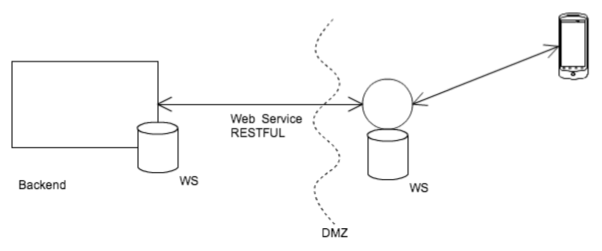
\includegraphics[width=10cm]{esquema_sistema_entrevista.png}
\caption{Esquema proporcionado por el analista durante la entrevista.}
\end{figure}
 
% Intervención del entrevistador
\paragraph{Diego} Se pregunta a Javier acerca del alcance que tiene dicho servicio, que limites de jurisdicción tiene dentro del término municipal.
 
% Intervención del responsable de operativa
\paragraph{Javier} Hay un limite de alcance, llega a la zona urbana y a la zona de núcleos rurales. No se limita sólo a zona urbana. Lo que ocurre es que para las zonas rurales hay un día a la semana. Las zonas rurales tienen su problemática aparte. Si no incluimos las zonas rurales, la puesta en producción va a ser más complicada. Nos recomienda hacer de las zonas rurales un sector más de las peticiones de servicio pero con la condición de que se les de sólo un día.  El motivo de que sólo se les de un día es debido a que las zonas rurales tienen una densidad de población más baja y la generación de residuos es más baja. Dentro de las zonas rurales, en el 99\% de los casos, hay una tipología de viviendas que permiten mantener el residuo una semana o dos al tratarse generalmente de parcelas grandes. Aunque en verano suele subir el número de peticiones de recogida en las zonas rurales, aunque sin cambiar la estructura funcional, esto es, sigue habiendo un solo día de recogida. Con un día de la semana, por el momento, suele ser suficiente.
 
% Intervención del entrevistador
\paragraph{Diego} Se pregunta acerca del número de peticiones por usuario en ubicaciones distintas.
 
% Intervención del responsable de operativa
\paragraph{Javier} Normalmente al día no se suele solicitar peticiones en diversas ubicaciones, nunca se ha dado el caso. Lo que si se suele dar es que haya mucho volumen de enseres y el mismo usuario solicite varias citas para el mismo punto de recogida, pero él personalmente nunca recuerda que se le hayan solicitado una petición por un usuario en diversos puntos.
 
% Intervención del analista
\paragraph{Enrique} Se nos recuerda que la aplicación debe desarrollarse en tres niveles
\begin{itemize}
\item Aplicación para dispositivo móvil (\textit{Android}).
\item  Servicio.
\item Aplicación simple de \textit{backend} para pruebas donde se muestre mediante una aplicación de escritorio simple la gestión de peticiones.
\end{itemize}
Inicialmente se hará una simulación de cómo funcionaría y posteriormente, cuando se lleve a producción el \text{backend}, será sustituido por el existente.
 
% Intervención del entrevistador
\paragraph{Diego} Se pregunta sobre la clasificación de zonas.
 
% Intervención del analista
\paragraph{Enrique} Dice que es muy simple y enumera las zonas : Centro, Río San Pedro, Las Canteras, Casines, Barrio Jarana, Meadero de la Reina y Zonas Rurales. Aunque en determinadas zonas, habiendo zonas rurales y urbanas, se distinguirían zonas de recogida ordinaria (diaria) y zonas de recogida especial (una vez a la semana). Se consideraría una primera versión y posteriormente, una versión de producción en la que se analice con más detenimiento la casuística.
 
 % Intervención del responsable de operativa
\paragraph{Javier} Sugiere que, en principio, para una primera versión quizás no sea tan importante dividir la localidad en 7 zonas sino en dos: zonas urbanas y zonas rurales. La casuística tampoco debe contemplar toda la casuística sino la que se contempla en el 90\% de los casos.

\paragraph{Diego}Finalmente se agradece su colaboración y se da por finalizada la entrevista. 
